\documentclass[spanish]{udpreport}
\usepackage[utf8]{inputenc}
\usepackage[spanish]{babel}
\graphicspath{{images/}}
\usepackage{graphicx}
\usepackage{multirow}
\usepackage{verbatim} 
\usepackage{upgreek} 

% Podemos establecer el logo de alguna entidad o dejar el de la UDP (defecto)
\setlogo{EITFI}

\title{Metodologia RUP}
\author{Christian López \\ Thomas Muñoz \\ Flavio Pallini}
\email{christian.lopeza@mail.udp.cl \\ thomas.munoz@mail.udp.cl }
\date{29 de agosto de 2017}

% Además podemos establecer la facultad y escuela
% los valores por defecto son los siguientes:
\udpschool{Escuela de Informática y Telecomunicaciones}
\udpfaculty{Facultad de Ingeniería y Ciencias}
\udpuniversity{Universidad Diego Portales}

\begin{document}
\maketitle

\tableofcontents
\listoffigures

\chapter{Introducción}
Hoy en día es casi imposible realizar un proyecto de software sin hacer uso de alguna metodología, ya que estos requieren de un manejo de muchas variables, métodos y procesos. Es por esto que para satisfacer estas necesidades se hace uso de la ingeniería de software como pauta a seguir cuando se quiere modelar la solución a un problema de software en una empresa.\par
La metodología RUP, es un proceso de desarrollo de software creado por \textit{Rational Software}, y actualmente propiedad de IBM, obteniendo el nombre de \textit{Rational Unified Process}.\par
Es uno de los métodos de desarrollo de software más utilizados para el análisis, implementación y documentación de sistemas orientados a objetos. Se caracteriza por no ser estático, ya que está compuesto por un conjunto de fases adaptables según la necesidad del cliente o avance del equipo de desarrollo.

\chapter{Explicación de Metodología}
Esta metodología permite dividir el proceso de desarrollo en cuatro grandes fases donde cada una incluye modelamiento del negocio, análisis, diseño, construcción, pruebas e implantación.

\section{¿Por qué utilizar RUP?}
\label{sec: Por que utilizar RUP}
RUP proporciona información sobre lo que puede esperarse de la tarea de desarrollo. Ofrece un glosario de terminología y una enciclopedia de conocimiento que le ayuda a comunicar sus necesidades de forma eficaz al equipo de  desarrollo de software. \par
Para un gestor o jefe de equipo, RUP proporciona  un proceso el cual le permite comunicarse de forma eficaz con el personal, gestionar la planificación y el control de su trabajo. Para un Diseñador, RUP proporciona una buena base de arquitectura y una gran cantidad de materiales con las que construir una definición de un proceso, lo que le permite configurar y ampliar dicha base como desee.

\section{¿Cuándo debo utilizar RUP?}
\label{sec: Cuando debo utilizar RUP}
Se utiliza RUP desde el inicio de  un proyecto de software, y puede seguir utilizándolo en los ciclos de desarrollo subsiguientes tiempo después de que le proyecto inicial haya terminado. \par
La forma de utilizar RUP varía para ajustarse a sus necesidades. Existen unas pocas consideraciones que determinarán cuando y como utilizar partes diferentes de RUP.
\begin{itemize}
\item Ciclo vital del proyecto(numero de iteraciones, longitud de cada fase)
\item Propósitos empresariales, visión, ámbito y riesgo del proyecto
\item Tamaño del esfuerzo de desarrollo de software
\end{itemize}
En la siguiente figura \ref{fig:grafico} muestra a través de un gráfico de complejidad de técnica y gestión:

\begin{figure}[h]
	\centering
	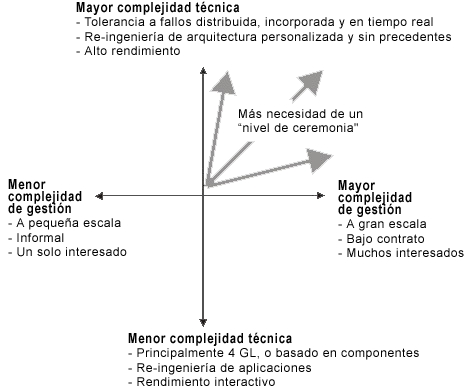
\includegraphics[width=0.7\textwidth]{RUP.png}
	\caption{\label{fig:grafico}Gráfico complejidad de técnica y gestión.}
\end{figure}

\section{Fases de la metodología RUP}
Las fases indican el énfasis que se da en el proyecto en un instante dado. Para capturar la dimensión temporal de un proyecto, RUP divide el proyecto en cuatro fases diferentes(ver figura \ref{fig:fases}):

\begin{figure}[!h]
	\centering
	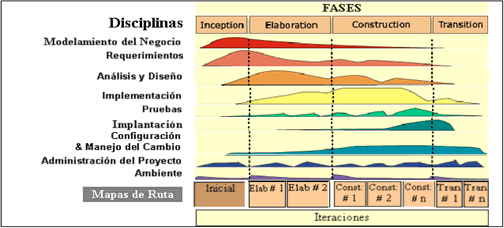
\includegraphics[width=0.8\textwidth]{fases.png}
	\caption{\label{fig:fases}Fases de RUP.}
\end{figure}

\begin{itemize}
\item Iniciación o Diseño: énfasis en el alcance del sistema
\item Preparación: énfasis en la arquitectura
\item Construcción: énfasis en el desarrollo
\item Transición: énfasis en la aplicación

\end{itemize}

\subsection{Fase de Inicio}
\label{subsec:inicio}
El objetivo preferente de esta fase es alcanzar un acuerdo entre todos los interesados respecto a los objetivos del ciclo vital del proyecto.
Es muy significativa la fase de inicio, pues son más arriesgados para los requisitos y para la actividad comercial y deben abordarse antes de que el proyecto pueda continuar.\par
La duracion de esto es generalmente corto y se utiliza para definir si es factible seguir y definir los riesgos. Un prototipo se puede hacer para que el cliente pruebe el software.\par


\subsection{Fase de elaboracion}
\label{subsec:elaboracion}
El proposito de esta fase es el establecimiento de una arquitectura de sistema para proporcionar una base estable para el diseño y la implementación en la fase de construccion. La arquitetura va evolucionando  a partir de una consideracion de requisitos mas significativos y  una valoracion a los riesgos.\par
Al final de la fase de elaboración se encuentra el segundo objectivo mas importante del proyecto que es el ciclo vital de la arquitectura. En esta se examina los objectivos y el ámbito del sistema detallado, la eleccion de arquitectura y la resolucion a los principales riesgos.

\subsection{Fase de Construcción}
\label{subsec:construccion}
El objectivo de la fase de construccion es aclarar lo requisitos restantes y completar el desarrolo del sistema basandose en la base de la arquitectura.
En esta fase sespone el énfasis en la gestion de los recursos y el control de la operaciones para poder optimizar los costes, la planificacion y la calidad.\par

\subsection{Fase de Transición}
En esta fase se garantiza que el software este diponicle para los usuarios finales, ademas se puede acarrear varias iteraciones e incluye las pruebas del producto en preparación para el release, asi como los ajustes menores basados en la informacion obtenida de los usuarios que han probado el software.\par
En este momento del ciclo vital, la informacion recibida de los usuarios debe centrarse especialmente en el ajuste del producto, las cuestiones de configuracion, instalacion y utilización.

\chapter{Aplicación en Canchapp}

\chapter{Conclusión}


%\listoftables


\end{document}

